\documentclass[11pt]{article}\usepackage{graphicx, color}
%% maxwidth is the original width if it is less than linewidth
%% otherwise use linewidth (to make sure the graphics do not exceed the margin)
\makeatletter
\def\maxwidth{ %
  \ifdim\Gin@nat@width>\linewidth
    \linewidth
  \else
    \Gin@nat@width
  \fi
}
\makeatother

\IfFileExists{upquote.sty}{\usepackage{upquote}}{}
\definecolor{fgcolor}{rgb}{0.2, 0.2, 0.2}
\newcommand{\hlnumber}[1]{\textcolor[rgb]{0,0,0}{#1}}%
\newcommand{\hlfunctioncall}[1]{\textcolor[rgb]{0.501960784313725,0,0.329411764705882}{\textbf{#1}}}%
\newcommand{\hlstring}[1]{\textcolor[rgb]{0.6,0.6,1}{#1}}%
\newcommand{\hlkeyword}[1]{\textcolor[rgb]{0,0,0}{\textbf{#1}}}%
\newcommand{\hlargument}[1]{\textcolor[rgb]{0.690196078431373,0.250980392156863,0.0196078431372549}{#1}}%
\newcommand{\hlcomment}[1]{\textcolor[rgb]{0.180392156862745,0.6,0.341176470588235}{#1}}%
\newcommand{\hlroxygencomment}[1]{\textcolor[rgb]{0.43921568627451,0.47843137254902,0.701960784313725}{#1}}%
\newcommand{\hlformalargs}[1]{\textcolor[rgb]{0.690196078431373,0.250980392156863,0.0196078431372549}{#1}}%
\newcommand{\hleqformalargs}[1]{\textcolor[rgb]{0.690196078431373,0.250980392156863,0.0196078431372549}{#1}}%
\newcommand{\hlassignement}[1]{\textcolor[rgb]{0,0,0}{\textbf{#1}}}%
\newcommand{\hlpackage}[1]{\textcolor[rgb]{0.588235294117647,0.709803921568627,0.145098039215686}{#1}}%
\newcommand{\hlslot}[1]{\textit{#1}}%
\newcommand{\hlsymbol}[1]{\textcolor[rgb]{0,0,0}{#1}}%
\newcommand{\hlprompt}[1]{\textcolor[rgb]{0.2,0.2,0.2}{#1}}%

\usepackage{framed}
\makeatletter
\newenvironment{kframe}{%
 \def\at@end@of@kframe{}%
 \ifinner\ifhmode%
  \def\at@end@of@kframe{\end{minipage}}%
  \begin{minipage}{\columnwidth}%
 \fi\fi%
 \def\FrameCommand##1{\hskip\@totalleftmargin \hskip-\fboxsep
 \colorbox{shadecolor}{##1}\hskip-\fboxsep
     % There is no \\@totalrightmargin, so:
     \hskip-\linewidth \hskip-\@totalleftmargin \hskip\columnwidth}%
 \MakeFramed {\advance\hsize-\width
   \@totalleftmargin\z@ \linewidth\hsize
   \@setminipage}}%
 {\par\unskip\endMakeFramed%
 \at@end@of@kframe}
\makeatother

\definecolor{shadecolor}{rgb}{.97, .97, .97}
\definecolor{messagecolor}{rgb}{0, 0, 0}
\definecolor{warningcolor}{rgb}{1, 0, 1}
\definecolor{errorcolor}{rgb}{1, 0, 0}
\newenvironment{knitrout}{}{} % an empty environment to be redefined in TeX

\usepackage{alltt}
\usepackage{natbib}
\usepackage{fullpage}
\usepackage{hyperref}
\usepackage{wrapfig,float,subfig}
\usepackage{graphicx}
\usepackage{amssymb}

% help with editing and coauthoring
\usepackage{todonotes}

\graphicspath{{figure/}}





\title{Signs of the Sine Illusion -- why we need to care}
\author{Susan Vanderplas, Heike Hofmann, probably include Di and Xiaoyue}

\begin{document}
\maketitle
\begin{abstract}
The sine illusion, which is part of a set of optical illusions which occur based on a conflict between a stimuli and the real-world situation which can cause similar stimuli, has a notable impact on perception of time-series data with a seasonal component. In this paper, we discuss the reasons for the illusion and various strategies which might be useful to break the illusion or reduce its' strength, demonstrating the presence of the illusion in real-world and theoretical situations. We also present data from user studies which demonstrate the dramatic effect the sine illusion can have on conclusions drawn from displayed data.
\end{abstract}
\tableofcontents
\section{Background and Introduction}
\todo[inline]{this is where we need to introduce the sine-illusion

and lay out the problem that we have with it from a statistical graphics side

then we sketch out a remedy

last paragraph is a sentence on the structure of the paper. 
}


In the perception literature, the phenomenon is known as part of a group of geometrical optical misperceptions classified as M\"uller-Lyer illusions \citep{day:1991}. Figure \ref{original} shows a reproduction of Bach's applet \citep{bach} displaying the sine illusion. The sine illusion is closely related to the line width phenomenon -- the line segments along the steepest slopes of the sine curve appear to be the shortest: ``The illusion is explained in terms of a perceptual compromise between the vertical extent and the greater overall dimensions of the section at the turn of the sine-wave figure and is thereby held to be the same in principle as the M\"uller-Lyer illusion." \citep{day:1991}.
M Bach's applet  gives the option to compensate the line length manually for its perceived shortcoming. The amount of compensation chosen turns out to be highly dependent on both the length of the vertical line segments and the amplitude of the sine function. The amplitude directly affects the slope -- the steeper  the slope the more compensation is necessary, see section \ref{distortion}  for a more detailed discussion and some results from a user study  \todo{could we start with our own data for the user study? that way we don't need IRB approval for now. data is in the data folder. I don't see any clear relationship, though/}.



\begin{figure}[hbtp]
\centering
\begin{minipage}{.495\textwidth}


{\centering \includegraphics[width=\maxwidth]{figure/fig-original} 

}




\end{minipage}\begin{minipage}{.495\textwidth}


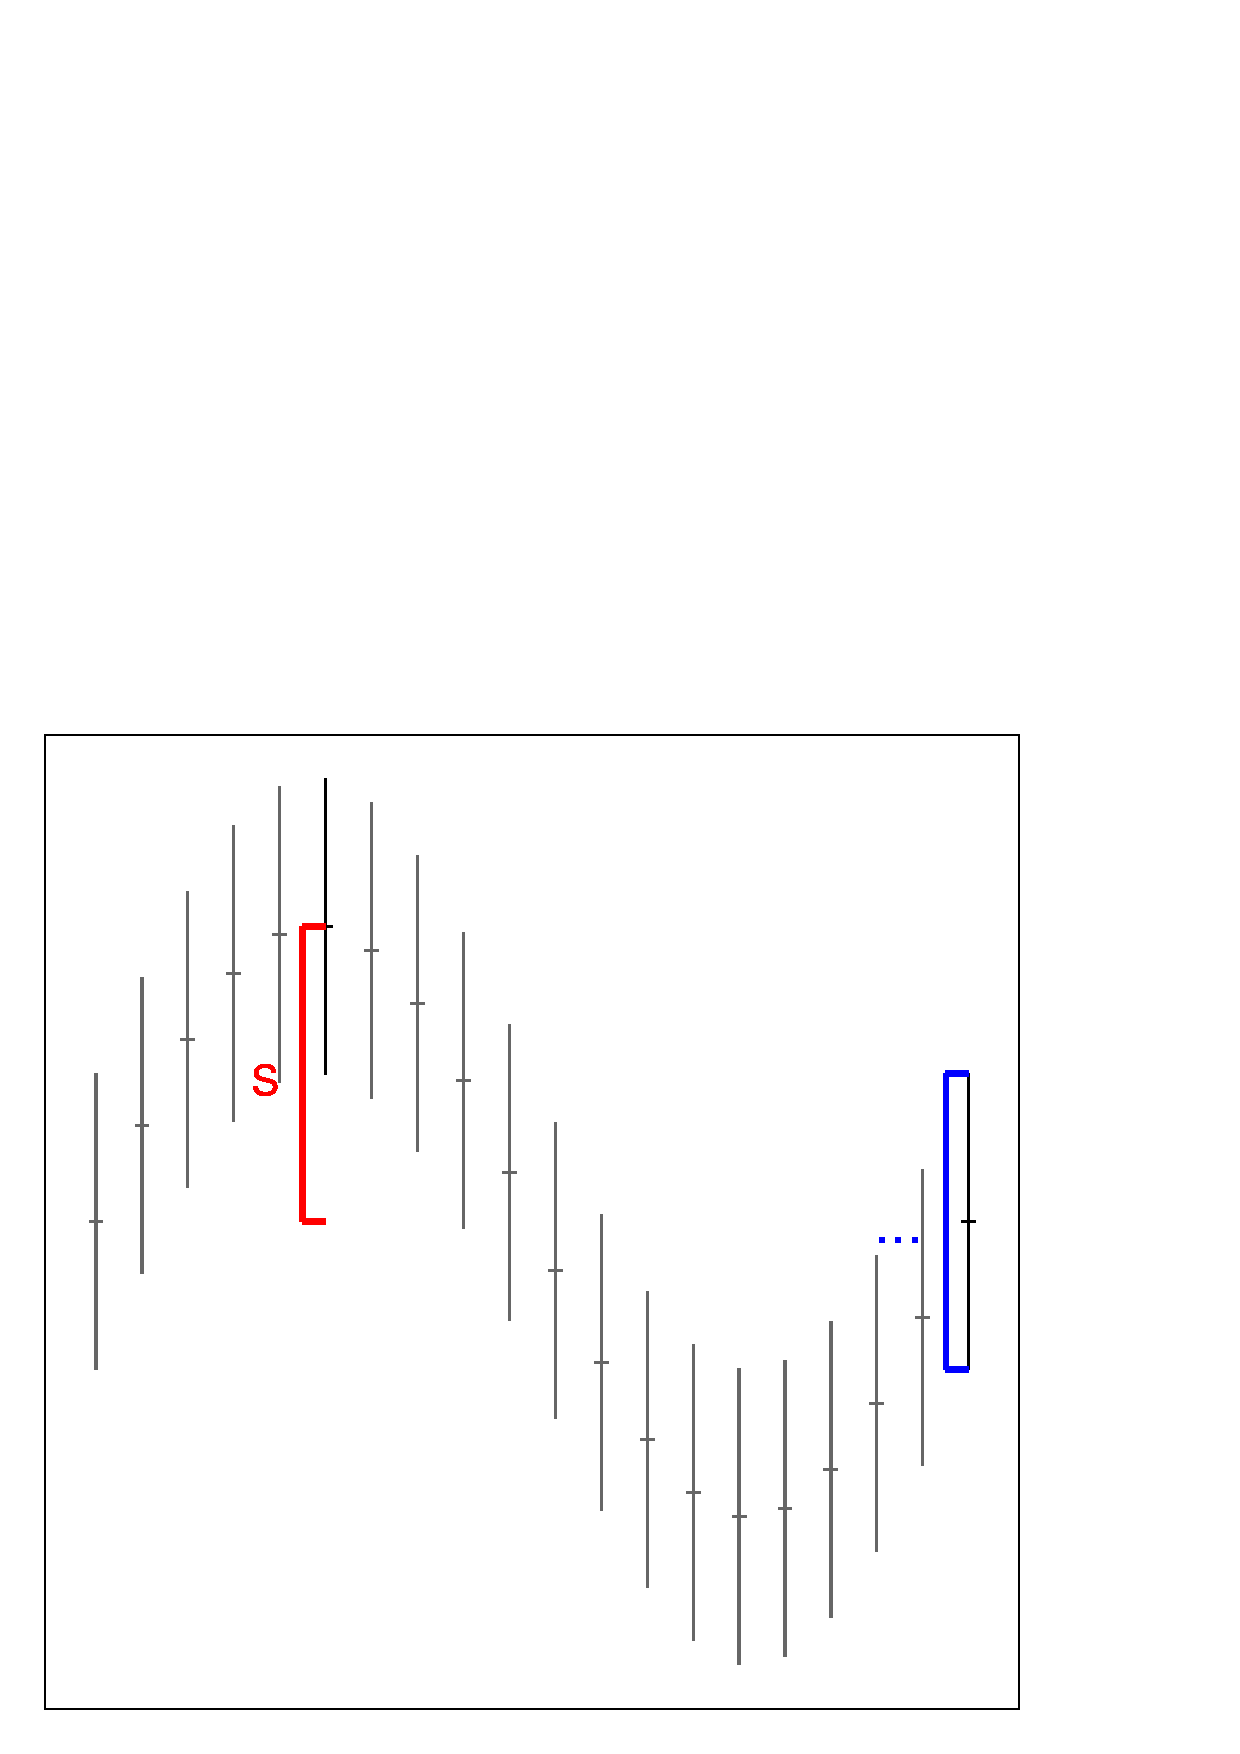
\includegraphics[keepaspectratio=true, width=\linewidth]{fig-original-redo.pdf}
\end{minipage}
\caption{\label{original}The original Sine Illusion. The regions of the graph in the peak and the valley appear to be composed of longer lines than the other regions. $s$ denotes the amplitude of the function, $\ell$ the length of the line segments.}
\end{figure}

\begin{figure}[hbtp]
\centering


{\centering \includegraphics[width=.5\linewidth]{figure/fig-originalgrid} 

}




\caption{\label{originalgrid} Horizontal grid lines do not help much in resolving the illusion, even though they provide a clear basis for comparison of line lengths.}
\end{figure}

\clearpage
\subsection*{Discussion of Sine Illusion}
Using the notation given in the applet, we assume a value $s$ for the sine amplitude, $\ell$ for the vertical length of line segments, and $\ell_c$ for the amount of compensation. 
The sine curve is then given by function $f$, written as 
\[
f(x) = s/2 \sin(x)
\]
for $x$ in $[-\pi, \pi]$. The slope of the sine curve is the steepest in its reflection point at $x=0$. We can calculate the slope as $f^\prime(x) = s/2 \cos(x)$, which in $x=0$ yields a slope of $s/2$.

These differences in the slope are the reason we perceive the lines to have different length, as we have an innate tendency to evaluate line or band widths orthogonally rather than vertically, as would be the mathematically correct way.

Orthogonal $w_o$ and vertical $w_v$ line widths are related -- the orthogonal line width depends on the angle (or, equivalently, the slope) of the line:
\begin{equation}\label{adjust}
w_o = w_v \cos \theta,
\end{equation}
where $\theta$ is the angle of the line with respect to the horizontal line.
\todo[inline]{Should we make the $w_o$ vs. b and $w_v$ vs. a terminology consistent?}
\begin{figure}[htbp]
\begin{center}
\includegraphics[width=0.3\linewidth]{images/linewidth}
\end{center}
\caption{\label{fig:linewidth}Sketch of line width assessments: (a) is showing  vertical width, (b) shows  width orthogonal to the slope. From previous surveys (we could cite Marie's survey here) we know that  observers associate line width more with  orthogonal width (b) than vertical width (a).}
\end{figure}
% 
% \todo[inline]{get the figures out of the knitr specification - you have much more control over the sizing that way.}

\begin{figure}[htbp]
\centering


\includegraphics[width=.5\linewidth, keepaspectratio=TRUE]{figure/fig-transform-illustration}
\caption{The perceived width orthogonal to the slope differs from the length of the lines.}
\end{figure}

One way to correct for the sine illusion is to make all slopes the same (by transforming the $x$ axis), another approach is to make the lines appear to be of the same height, by adjusting their lengths to maintain a constant orthogonal width. This is the approach that we pursue when transforming the $Y$ values. 
\clearpage
\section{Correction Approaches to the Sine Illusion}

Web Link: \url{http://www.michaelbach.de/ot/sze_sineIllusion/index.html}
\begin{quote}
The original authors \citep{day:1991} write in their abstract: The illusion is explained in terms of a perceptual compromise between the vertical extent and the greater overall dimensions of the section at the turn of the sine-wave figure and is thereby held to be the same in principle as the M\"uller-Lyer illusion.
\end{quote}

\begin{figure}[h!tbp]\centering


\includegraphics[width=.5\linewidth, keepaspectratio=TRUE]{figure/fig-ribbon-illusion}
\caption{Experience with real-world objects suggests that the data are most similar to a slightly angled top view of a 3-dimensional strip such as a ribbon. Even though the sine illusion lines are not angled, the brain interprets the physiological stimuli within this context. This produces a conflict between past experience and the present perception that leads to the illusion.}
\end{figure}

As in the M\"uller-Lyer illusion, the perceptual experience is influenced by the context in which similar stimuli exist in real world situations. One other common illusion of this sort is the Ames Room illusion (\url{http://en.wikipedia.org/wiki/Ames_room}), where ambiguous stimuli are perceived as resulting from situations that occur in the real world, even when those perceptions are misleading. This is in general an optimal processing strategy, as the vast majority of visual stimuli conform to the brain's expectations, however, it does lead to certain visual ``bugs" that we must work around when designing graphics.
 
\clearpage
\begin{subsection}{Data Setup}
\todo[inline]{Describe the setup of the data in words and leave out the code from the paper.}
We begin with lines of length 2 evenly spaced along the x-axis, where the center of the vertical line is at $y = sin(x)$. For this example, the amplitude $s$ = 1 and the line length $\ell = 2$. Our goal is to break the sine illusion by transforming the line length, $f(\ell) = \ell + \ell_c$ so that the perceived width is constant. 

\end{subsection}

\begin{subsection}{Transformation of Y values}
This approach aims to extend the orthogonal width, which onlookers generally evaluate,  to the amount of the vertical width, which we want to represent. 
For that, we multiply the vertical width by a factor of $1/\cos\theta$, where $\theta$ is the angle under which the line is drawn. This angle is given by the slope of the function, mathematically we know that in position $x$ the angle $\theta(x)$ of function $f(x)$ is given as:
\[
\tan \theta (x) = f^\prime (x).
\]
We only distinguish the size, not the sign of the angle, which gives us an overall correction factor for the line width in vertical direction of 
\begin{equation}\label{correction1}
atan \left(\cos \left| f^\prime (x) \right|\right) ^{-1}
\end{equation}







\begin{figure}[htbp]\centering



\subfloat[Aspect Ratio of .5]{\includegraphics[width=.32\linewidth,keepaspectratio=TRUE]{figure/fig-ytransform1-plot1}}
\subfloat[Aspect ratio of 1]{\includegraphics[width=.32\linewidth,keepaspectratio=TRUE]{figure/fig-ytransform1-plot2}}
\subfloat[Aspect ratio of 2]{\includegraphics[width=.32\linewidth,keepaspectratio=TRUE]{figure/fig-ytransform1-plot3}}
\caption{Changing aspect ratios changes the strength of the illusion and the effectiveness of the transformation}
\end{figure}
% 
% <<echo=FALSE, fig=TRUE, results='asis',out.width=".48\\textwidth">>=
% qplot(x=x, xend=x, y = y2start, yend=y2end, colour=I("blue"), geom="segment", main="Transformed Length") +
%   #geom_line(aes(x=x, y=cos(2*x)), colour=I("red")) +
%   #geom_segment(aes(x = 0, xend=2*pi, y=0, yend=0), colour="black") + 
%   theme(plot.background=element_blank(), panel.grid.major=element_blank(), 
%        panel.grid.minor=element_blank(), panel.background=element_blank())+ylim(c(-3, 3))
% qplot(x=x, xend=x, y = y2start, yend=y2end, colour=I("blue"), geom="segment", main="Transformed Length") +
%   #geom_line(aes(x=x, y=cos(2*x)), colour=I("red")) +
%   #geom_segment(aes(x = 0, xend=2*pi, y=0, yend=0), colour="black") + 
%   theme(plot.background=element_blank(), panel.grid.major=element_blank(), 
%        panel.grid.minor=element_blank(), panel.background=element_blank())+ylim(c(-10, 10))
% @
% 
% <<echo=FALSE, fig=TRUE, results='asis',out.width=".48\\textwidth">>=
% qplot(x=x, xend=x, y = y2start-sin(x), yend=y2end-sin(x), colour=I("blue"), geom="segment", main="Transformed Length, mean=0") +
%   #geom_line(aes(x=x, y=cos(2*x)), colour=I("red")) +
%   #geom_segment(aes(x = 0, xend=2*pi, y=0, yend=0), colour="black") + 
%   theme(plot.background=element_blank(), panel.grid.major=element_blank(), 
%        panel.grid.minor=element_blank(), panel.background=element_blank())+ylim(c(-3, 3))
% qplot(x=1:length(l), y=l1, geom="line", main="L vs L*") + 
%   geom_segment(aes(x=0, xend=length(l), y=l[1], yend=l[1]), colour="black", linetype=2)
% @


\begin{figure}[hbtp]


{\centering \includegraphics[width=.49\textwidth]{figure/fig-fixingit1} 
\includegraphics[width=.49\textwidth]{figure/fig-fixingit2} 

}




\caption{\label{firstfix} First fix of the sine illusion by using the factor of $1/cos(atan(|f^\prime(x)|))$ for adjusting the vertical extent of the lines.}
\end{figure}

\begin{figure}
\centering
\begin{knitrout}
\definecolor{shadecolor}{rgb}{0.969, 0.969, 0.969}\color{fgcolor}

{\centering \includegraphics[width=0.49\textwidth]{figure/fig-secondfix1} 
\includegraphics[width=0.49\textwidth]{figure/fig-secondfix2} 

}



\end{knitrout}

\caption{\label{secondfix} Aspect ratio seems to be a scalar in the correction factor.}
\end{figure}

\begin{figure}
\centering
\begin{knitrout}
\definecolor{shadecolor}{rgb}{0.969, 0.969, 0.969}\color{fgcolor}

{\centering \includegraphics[width=0.49 \textwidth]{figure/fig-thirdfix1} 
\includegraphics[width=0.49 \textwidth]{figure/fig-thirdfix2} 

}



\end{knitrout}

\caption{\label{thirdfix} The ratio of the length of the line to amplitude of the function needs to be included in the correction. Here, the amplitude is still 1, but the length of the line is 5. The correction factor leads to a massive over correction that makes the function almost unrecognizable. The plot on the left is uncorrected, the plot on the right is `corrected'.}
\end{figure}


\end{subsection}\clearpage
\section{Distortion} \label{distortion}
place holder
\section{Application: Simulation}
\begin{knitrout}
\definecolor{shadecolor}{rgb}{0.969, 0.969, 0.969}\color{fgcolor}\begin{kframe}
\begin{alltt}
x <- \hlfunctioncall{rep}(\hlfunctioncall{seq}(0, 2 * pi * 10, length = 120), each = 100)
y <- \hlfunctioncall{rnorm}(n = \hlfunctioncall{length}(x), mean = \hlfunctioncall{sin}(x), sd = 0.2)
\hlfunctioncall{qplot}(x, y, geom = \hlstring{"jitter"})
\end{alltt}
\end{kframe}

{\centering \includegraphics[width=\maxwidth]{figure/fig-sine} 

}



\end{knitrout}


\begin{knitrout}
\definecolor{shadecolor}{rgb}{0.969, 0.969, 0.969}\color{fgcolor}\begin{kframe}
\begin{alltt}
x <- \hlfunctioncall{rep}(\hlfunctioncall{seq}(0, 2 * pi * 10, length = 120), each = 100)
y <- \hlfunctioncall{rnorm}(n = \hlfunctioncall{length}(x), mean = 5 * \hlfunctioncall{sin}(x/20) + \hlfunctioncall{sin}(x), sd = 0.2)
\hlfunctioncall{qplot}(x, y, geom = \hlstring{"jitter"})
\end{alltt}
\end{kframe}

{\centering \includegraphics[width=\maxwidth]{figure/fig-sinetrend} 

}



\end{knitrout}


\section{Application: USHCN Data}



\begin{figure}[hbtp]
\centering
\begin{knitrout}
\definecolor{shadecolor}{rgb}{0.969, 0.969, 0.969}\color{fgcolor}

{\centering \includegraphics[width=\textwidth]{figure/fig-rawtemp} 

}



\end{knitrout}

% \includegraphics[width=\textwidth]{monthly-temps}
\caption{\label{raw-temp}Raw monthly maximum temperatures (in Celsius) between 1980 and 2012 at 1218 stations across the US. The blue line shows fitted temperatures from a baseline model. The plot suggests that the model fails to capture the more extreme values in summer and winter. }
\end{figure}
\begin{figure}[hbtp]\centering
\begin{knitrout}
\definecolor{shadecolor}{rgb}{0.969, 0.969, 0.969}\color{fgcolor}

{\centering \includegraphics[width=\textwidth]{figure/fig-boxtemp} 

}



\end{knitrout}


\caption{\label{box-temp}Monthly boxplot of maximum temperatures (in Celsius) between 1980 and 1995 at 1218 stations across the US. The sine illusion is less powerful but still visible in three locations:  the box area of the boxes,  the whiskers, and in the outliers.}
\end{figure}
\begin{figure}[hbtp]
\centering
\begin{knitrout}
\definecolor{shadecolor}{rgb}{0.969, 0.969, 0.969}\color{fgcolor}

{\centering \includegraphics[width=\textwidth]{figure/fig-residtemp} 

}



\end{knitrout}

% \includegraphics[width=\textwidth]{monthly-resid-temps}
\caption{\label{resid-temp}Residual monthly temperatures (in Celsius) from the baseline model fit. The original impression of smaller deviations during Spring and Fall is now almost gone: Winters have larger negative residuals, while Summers have larger positive ones. }
\end{figure}

Figures \ref{raw-temp} and \ref{resid-temp} show temperature data from 1218 stations across the US. The first plot shows raw temperatures, the second residuals from a `baseline' model. The caption for the raw temperature plot suggests that the baseline model is not quitable to capture all of the variability in summer and winter peaks. However, the model used is actually based on averages in each time point. This model is not  susceptible to shrinking values, and it is our perception of the plot rather than the data that makes us see any higher variability in the peaks. After removing the averages in figure \ref{resid-temp} the impression of higher variability in the peaks is gone with the exception of a few outliers.

\bibliographystyle{asa}
% argument is your BibTeX string definitions and bibliography database(s)
\bibliography{references}

\end{document}


\begin{subsection}{Transformation of $X$ Values}
\todo[inline]{Could you try to write the correction factor out in terms of a formula? - I still think that all of the lines should appear under the same slope, which means that the result would need to be an up/down triangle, like we had before. I'm a bit worried about the `fudge' factor $a$ -- let's first use a correction factor that we can derive mathematically from counteracting the line illusion and then allow some fudging. }
In order to counteract the illusion of changing line length, we can slightly transform the $X$ values, narrowing the distance between values at the peak and trough of the curve and widening the distance between values at the inflection point. If we alter the $X$ axis such that $\triangle X^\ast = c*a(\cos(2x)+1)$, where $\triangle X = c$ is the distance between two evenly spaced $X$ points, the illusion's effect is broken and all $y$ values appear to be approximately the same length. Consistent with the hypothesis that the apparent line length is dependent on the slope of the tangent line, changing $\triangle x$ reduces the apparent length discrepancy $\triangle y$ significantly.
\begin{figure}[H]\centering



{\centering \includegraphics[width=.31\textwidth]{figure/fig-xtransform1} 
\includegraphics[width=.31\textwidth]{figure/fig-xtransform2} 

}





\end{figure}
\end{subsection}

\begin{subsection}{Exploration of Effect with Random Data}
If we use randomly spaced x, does the effect still hold?
\begin{knitrout}
\definecolor{shadecolor}{rgb}{0.969, 0.969, 0.969}\color{fgcolor}\begin{kframe}
\begin{alltt}
\hlfunctioncall{library}(ggplot2)

x <- \hlfunctioncall{runif}(100, 0, 2 * pi)
x <- x[\hlfunctioncall{order}(x)]
l <- \hlfunctioncall{rep}(1, 100)
ystart <- \hlfunctioncall{sin}(x) - 0.5 * l
yend <- \hlfunctioncall{sin}(x) + 0.5 * l

a2 <- \hlfunctioncall{max}(\hlfunctioncall{diff}(ystart)/\hlfunctioncall{diff}(x) * (2 * pi/100))
l3 <- l + a2 * \hlfunctioncall{cos}(2 * x)
y3start <- \hlfunctioncall{sin}(x) - 0.5 * l3
y3end <- \hlfunctioncall{sin}(x) + 0.5 * l3
\end{alltt}
\end{kframe}
\end{knitrout}

\begin{knitrout}
\definecolor{shadecolor}{rgb}{0.969, 0.969, 0.969}\color{fgcolor}

{\centering \includegraphics[width=.48\textwidth]{figure/fig-unnamed-chunk-21} 
\includegraphics[width=.48\textwidth]{figure/fig-unnamed-chunk-22} 

}



\end{knitrout}


If we use randomly varying line lengths, with evenly spaced x, does the effect hold?
In particular, can we use an improvised (from the data) correction factor with uneven x spacing?
\begin{knitrout}
\definecolor{shadecolor}{rgb}{0.969, 0.969, 0.969}\color{fgcolor}\begin{kframe}
\begin{alltt}
x <- \hlfunctioncall{seq}(0, 2 * pi, length = 100)
l <- \hlfunctioncall{rep}(1, 100)
ystart <- \hlfunctioncall{sin}(x) - 0.5 * l
yend <- \hlfunctioncall{sin}(x) + 0.5 * l
a <- \hlfunctioncall{max}(\hlfunctioncall{diff}(ystart))
sd1 <- 0.1
l4 <- \hlfunctioncall{rnorm}(100, 1, sd1)
l5 <- l4 + a * \hlfunctioncall{cos}(2 * x)
y4start <- \hlfunctioncall{sin}(x) - 0.5 * l4
y4end <- \hlfunctioncall{sin}(x) + 0.5 * l4
y5start <- \hlfunctioncall{sin}(x) - 0.5 * l5
y5end <- \hlfunctioncall{sin}(x) + 0.5 * l5
\end{alltt}
\end{kframe}
\end{knitrout}

With sd=0.1, the illusion seems to hold and the correction (on the underlying sine distribution) does seem to mitigate the illusion to a small degree. 

\begin{knitrout}
\definecolor{shadecolor}{rgb}{0.969, 0.969, 0.969}\color{fgcolor}

{\centering \includegraphics[width=.48\textwidth]{figure/fig-unnamed-chunk-41} 
\includegraphics[width=.48\textwidth]{figure/fig-unnamed-chunk-42} 

}



\end{knitrout}


\begin{knitrout}
\definecolor{shadecolor}{rgb}{0.969, 0.969, 0.969}\color{fgcolor}\begin{kframe}
\begin{alltt}
sd2 <- 0.2
l6 <- \hlfunctioncall{rnorm}(100, 1, sd2)
y6start <- \hlfunctioncall{sin}(x) - 0.5 * l6
y6end <- \hlfunctioncall{sin}(x) + 0.5 * l6
l7 <- l6 + a * \hlfunctioncall{cos}(2 * x)
y7start <- \hlfunctioncall{sin}(x) - 0.5 * l7
y7end <- \hlfunctioncall{sin}(x) + 0.5 * l7
\end{alltt}
\end{kframe}
\end{knitrout}


With sd=0.2, the illusion doesn't hold quite as strongly, and the correction (on the underlying sine distribution) similarly doesn't seem as effective. 

\begin{knitrout}
\definecolor{shadecolor}{rgb}{0.969, 0.969, 0.969}\color{fgcolor}

{\centering \includegraphics[width=.48\textwidth]{figure/fig-unnamed-chunk-61} 
\includegraphics[width=.48\textwidth]{figure/fig-unnamed-chunk-62} 

}



\end{knitrout}


\paragraph{Points}
Returning to the data presentation, does the sine illusion hold when data are presented as points instead of segments?
\begin{knitrout}
\definecolor{shadecolor}{rgb}{0.969, 0.969, 0.969}\color{fgcolor}\begin{kframe}
\begin{alltt}
x <- \hlfunctioncall{seq}(0, 2 * pi, length = 100)
l <- \hlfunctioncall{rep}(1, \hlfunctioncall{length}(x))
ystart <- \hlfunctioncall{sin}(x) - 0.5 * l
yend <- \hlfunctioncall{sin}(x) + 0.5 * l
a <- \hlfunctioncall{max}(\hlfunctioncall{diff}(ystart))
l1 <- l + a * \hlfunctioncall{cos}(2 * x)
y1start <- \hlfunctioncall{sin}(x) - 0.5 * l1
y1end <- \hlfunctioncall{sin}(x) + 0.5 * l1
\end{alltt}
\end{kframe}
\end{knitrout}

\begin{knitrout}
\definecolor{shadecolor}{rgb}{0.969, 0.969, 0.969}\color{fgcolor}

{\centering \includegraphics[width=.48\textwidth]{figure/fig-unnamed-chunk-81} 
\includegraphics[width=.48\textwidth]{figure/fig-unnamed-chunk-82} 

}



\end{knitrout}

After trying 0.0634, $\pi\times$0.0634, and  $2\pi\times$0.0634, I cannot seem to find a transformation that removes the illusion for points without any connecting line. It may be that a transformation in both x and y (or just in x) is required, as there is no dominant visual cue as to in which direction distance should be measured.
\paragraph{Line Graphs} The illusion also appears to hold for line graphs, but does not seem to be entirely mitigated by the correction factor.


\begin{knitrout}
\definecolor{shadecolor}{rgb}{0.969, 0.969, 0.969}\color{fgcolor}

{\centering \includegraphics[width=.48\textwidth]{figure/fig-unnamed-chunk-101} 
\includegraphics[width=.48\textwidth]{figure/fig-unnamed-chunk-102} 

}



\end{knitrout}

\begin{knitrout}
\definecolor{shadecolor}{rgb}{0.969, 0.969, 0.969}\color{fgcolor}

{\centering \includegraphics[width=.48\textwidth]{figure/fig-unnamed-chunk-111} 
\includegraphics[width=.48\textwidth]{figure/fig-unnamed-chunk-112} 

}



\end{knitrout}



3*a seems to be the optimal correction, perhaps because of the additional illusion of roundness (proxy to pi)? Additionally, the correction factor becomes noticable at the edges of the graph, when the roundness illusion ceases to exist. I'm not sure how to avoid that realization - possibly fade line color to grey?

\begin{knitrout}
\definecolor{shadecolor}{rgb}{0.969, 0.969, 0.969}\color{fgcolor}

{\centering \includegraphics[width=.48\textwidth]{figure/fig-unnamed-chunk-131} 
\includegraphics[width=.48\textwidth]{figure/fig-unnamed-chunk-132} 

}



\end{knitrout}


Without the sine function for the mean, the increased correction size is clear: 

\begin{knitrout}
\definecolor{shadecolor}{rgb}{0.969, 0.969, 0.969}\color{fgcolor}

{\centering \includegraphics[width=.48\textwidth]{figure/fig-unnamed-chunk-141} 
\includegraphics[width=.48\textwidth]{figure/fig-unnamed-chunk-142} 

}



\end{knitrout}

\end{subsection}
